\chapter{Testowanie aplikacji}
\label{cha:testowanieAplikacji}
Testowanie aplikacji ma na celu sprawdzenie poprawności działania kluczowych funkcji systemu oraz weryfikację, czy spełnione zostały wszystkie wymagania funkcjonalne i niefunkcjonalne. Proces testowania przeprowadzono ręcznie na różnych scenariuszach użytkowania zarówno po stronie klienta, jak i administratora. Sprawdzano m.in. rejestrację, logowanie, operacje na danych, zarządzanie sprzętem, rezerwacjami oraz generowanie dokumentów.

\section{Testowanie procesu uwierzytelniania użytkownika}
\label{sec:testlogowania}
W tej części przetestowano proces uwierzytelniania użytkownika, który obejmuje zarówno rejestrację nowych kont, jak i logowanie do aplikacji przez użytkownika oraz administratora. Celem testów było sprawdzenie poprawności działania formularzy oraz zabezpieczeń związanych z danymi wejściowymi.
\par
Testy obejmowały:
\begin{enumerate}%[1)]
\item Logowanie z prawidłowymi danymi użytkownika oraz admina;
\item Testowanie poprawnośći walidacji formularza;
\item Próba rejestracji użytkownika o istniejącej już nazwie użytkownika;
\item Logowanie przy błędnym loginie lub haśle;
\item Przykłady występujących błędów poniżej.
\end{enumerate}
Logowanie i rejestracja z poprawnymi danymi przebiegło pomyślnie, a w przypadku nie wypełnienia wszystkich pól pojawiał się komunikat „Wszystkie pola muszą być uzupełnione!”
\vspace{-0.2cm}
\begin{figure}[!htbp]
    \centering
    \includegraphics[width=0.5\linewidth, keepaspectratio]{figures/uzytkownikotejsamejnazwie.png}
    \caption{Próba rejestracji użytkownika o istniejącej już nazwie użytkownika}
    \label{fig:uzytkownikotejsamejNazwie}
    \small{Źródło: Opracowanie własne}
\end{figure}

\vspace{-0.2cm}
\begin{figure}[!htbp]
    \centering
    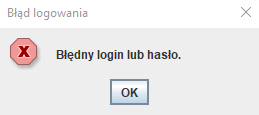
\includegraphics[width=0.5\linewidth, keepaspectratio]{figures/blednyloginlubhaslo.png}
    \caption{Próba logowania przy błędnym loginie lub haśle}
    \label{fig:blednyloginhaslo}
    \small{Źródło: Opracowanie własne}
\end{figure}
\clearpage

\section{Scenariusze testowania funkcjonalności rezerwacji sprzętu przez użytkownika}
\label{sec:rezerwacjaSprzetuTest}
Testy obejmowały:
\begin{enumerate}%[1)]
\item Wybór sprzętu z listy oraz weryfikację dostępności. System nie pozwala na złożenie rezerwacji bez wcześniejszego wskazania sprzętu – brak wyboru skutkuje komunikatem;
\item Wyznaczenie okresu rezerwacji oraz obliczenie kosztu. Po wskazaniu dat „od” i „do” użytkownik zobowiązany jest kliknąć przycisk „Oblicz Koszt”, aby system przeliczył wartość rezerwacji na podstawie ceny dziennej. Brak tej operacji uniemożliwia przejście do finalizacji;
\item Zabezpieczenie przed próbą rezerwacji bez wymaganych działań. W przypadku próby rezerwacji bez zaznaczenia sprzętu bądź bez wcześniejszego obliczenia kwoty, system wyświetla stosowne komunikaty ostrzegawcze („Wybierz sprzęt!”, „Najpierw oblicz kwotę!”);
\item Po spełnieniu wszystkich wymaganych warunków, proces rezerwacji przebiega prawidłowo;
\item Przykłady występujących komunikatów poniżej.
\end{enumerate}

\vspace{-0.2cm}
\begin{figure}[!htbp]
    \centering
    \includegraphics[width=0.5\linewidth, keepaspectratio]{figures/wybierzSprzet.png}
    \caption{Próba przejścia dalej bez zaznaczenia sprzętu}
    \label{fig:niezaznaczonySprzet}
    \small{Źródło: Opracowanie własne}
\end{figure}

\vspace{-0.2cm}
\begin{figure}[!htbp]
    \centering
    \includegraphics[width=0.5\linewidth, keepaspectratio]{figures/najpierObliczKwote.png}
    \caption{Próba przejścia dalej przy nie obliczeniu kwoty}
    \label{fig:brakObliczonejKwoty}
    \small{Źródło: Opracowanie własne}
\end{figure}

\section{Testowanie funkcjonalności panelu administratora}
\label{sec:TestowanieFunkcjonalnosci }
Testowanie panelu administratora miało na celu weryfikację poprawności działania głównych funkcji zarządzania użytkownikami, sprzętem oraz rezerwacjami. Sprawdzono, czy wszystkie akcje dostępne dla administratora wykonują się zgodnie z założeniami oraz czy interfejs prawidłowo reaguje na dane wejściowe.
\subsection{Panel zarządzania użytkownikami}
Wyświetlanie listy zarejestrowanych użytkowników działa poprawnie. Po kliknięciu przycisku usunięcia danego użytkownika, pojawia się komunikat z prośbą o potwierdzenie tej operacji, co zapobiega przypadkowemu usunięciu konta.
\subsection{Panel zarządzania sprzętem}
Walidacja formularza dodawania i edycji sprzętu działa prawidłowo – system uniemożliwia zapisanie danych w przypadku błędnie wypełnionych pól. Edycja danych sprzętu na podstawie ID przebiega bezproblemowo. Podczas próby usunięcia sprzętu wyświetlany jest komunikat z prośbą o potwierdzenie, co zabezpiecza przed przypadkowym usunięciem.
\subsection{Panel zarządzania rezerwacjami}
Funkcjonalność akceptowania i odrzucania rezerwacji działa prawidłowo — administrator ma możliwość skutecznego zarządzania zgłoszeniami użytkowników.
\subsection{Panel zarządzania wypożyczeniami}
Testowanie panelu Zarządzanie wypożyczeniami przebiegło pomyślnie. Generowanie paragonu działa poprawnie — system tworzy plik PDF po zaznaczeniu rezerwacji. Usuwanie również funkcjonuje prawidłowo, z komunikatem potwierdzającym przed wykonaniem operacji.

\section{Podsumowanie testowania aplikacji}
Przeprowadzone testy potwierdziły poprawność działania wszystkich funkcji aplikacji po stronie zarówno użytkownika, jak i administratora. Zweryfikowano proces rejestracji, logowania, dokonywania rezerwacji, zarządzania sprzętem oraz operacji administracyjnych. Wszystkie funkcjonalności – w tym walidacja danych, generowanie dokumentów PDF, usuwanie z potwierdzeniem oraz akceptacja rezerwacji – działały zgodnie z założeniami. 